\section{Summary \& Limitations}
\begin{frame}{}
    \LARGE Diffusion Models: \textbf{Summary \& Limitations}
\end{frame}

\begin{frame}{Summary}
    \begin{itemize}
        \item Diffusion models add noise to data and learn to reverse it
        \item Core task: Predict noise at different steps
        \item Training is efficient; Sampling is iterative and slow
        \item U-Nets with attention are the winning architecture
    \end{itemize}
\end{frame}


\begin{frame}{The Generative AI Landscape}
\begin{figure}
    \centering
    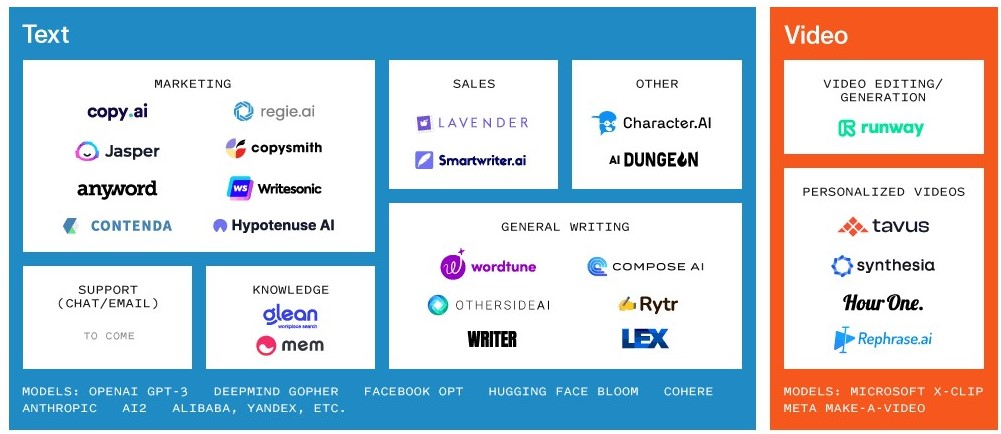
\includegraphics[height=0.9\textheight, width=1.05\textwidth, keepaspectratio]{images/diffusion/gen_ai_landscape.jpg}
\end{figure}
\footnotetext{\href{https://twitter.com/sonyatweetybird/status/1584580362339962880?cxt=HHwWgMCq9bXcx_0rAAAA}{Sonya Huang (@sonyatweetybird)}}
\end{frame}

\begin{frame}{The Generative AI Landscape}
\begin{figure}
    \centering
    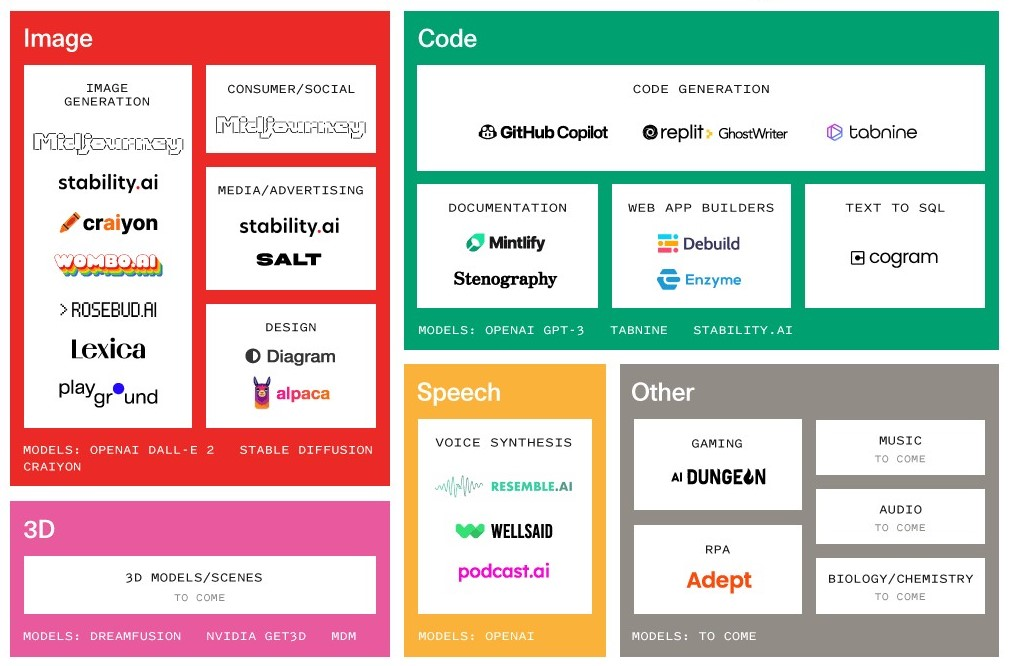
\includegraphics[height=0.9\textheight, width=1.05\textwidth, keepaspectratio]{images/diffusion/gen_ai_landscape_2.jpg}
\end{figure}
\footnotetext{\href{https://twitter.com/sonyatweetybird/status/1584580362339962880?cxt=HHwWgMCq9bXcx_0rAAAA}{Sonya Huang (@sonyatweetybird)}}
\end{frame}


\begin{frame}{Limitations}
    \begin{itemize}
        \item \textbf{Slow sampling} – iterative process
        \item \textbf{Data-heavy} – needs lots of varied data
        \item \textbf{Distribution miss} – struggles in tails of data
        \item \textbf{Compute needs} – high GPU/time investment
        \item \textbf{Misinformation concerns} – used in deepfake creation
    \end{itemize}
\end{frame}
